\documentclass[12pt,letterpaper]{article}
\usepackage{graphicx,textcomp}
\usepackage{natbib}
\usepackage{setspace}
\usepackage{fullpage}
\usepackage{color}
\usepackage[reqno]{amsmath}
\usepackage{amsthm}
\usepackage{fancyvrb}
\usepackage{amssymb,enumerate}
\usepackage[all]{xy}
\usepackage{endnotes}
\usepackage{lscape}
\newtheorem{com}{Comment}
\usepackage{float}
\usepackage{hyperref}
\newtheorem{lem} {Lemma}
\newtheorem{prop}{Proposition}
\newtheorem{thm}{Theorem}
\newtheorem{defn}{Definition}
\newtheorem{cor}{Corollary}
\newtheorem{obs}{Observation}
\usepackage[compact]{titlesec}
\usepackage{dcolumn}
\usepackage{tikz}
\usetikzlibrary{arrows}
\usepackage{multirow}
\usepackage{xcolor}
\newcolumntype{.}{D{.}{.}{-1}}
\newcolumntype{d}[1]{D{.}{.}{#1}}
\definecolor{light-gray}{gray}{0.65}
\usepackage{url}
\usepackage{listings}
\usepackage{color}

\definecolor{codegreen}{rgb}{0,0.6,0}
\definecolor{codegray}{rgb}{0.5,0.5,0.5}
\definecolor{codepurple}{rgb}{0.58,0,0.82}
\definecolor{backcolour}{rgb}{0.95,0.95,0.92}

\lstdefinestyle{mystyle}{
	backgroundcolor=\color{backcolour},   
	commentstyle=\color{codegreen},
	keywordstyle=\color{magenta},
	numberstyle=\tiny\color{codegray},
	stringstyle=\color{codepurple},
	basicstyle=\footnotesize,
	breakatwhitespace=false,         
	breaklines=true,                 
	captionpos=b,                    
	keepspaces=true,                 
	numbers=left,                    
	numbersep=5pt,                  
	showspaces=false,                
	showstringspaces=false,
	showtabs=false,                  
	tabsize=2
}
\lstset{style=mystyle}
\newcommand{\Sref}[1]{Section~\ref{#1}}
\newtheorem{hyp}{Hypothesis}

\title{Problem Set 1}
\date{Due: October 8, 2026}
\author{Applied Stats/Quant Methods 1}

\begin{document}
	\maketitle
	
	\section*{Instructions}
	\begin{itemize}
	\item Please show your work! You may lose points by simply writing in the answer. If the problem requires you to execute commands in \texttt{R}, please include the code you used to get your answers. Please also include the \texttt{.R} file that contains your code. If you are not sure if work needs to be shown for a particular problem, please ask.
\item Your homework should be submitted electronically on GitHub.
\item This problem set is due before 23:59 on Thursday October 8, 2026. No late assignments will be accepted.
	\end{itemize}
	
	\vspace{1cm}
	\section*{Question 1: Education}

A school counselor was curious about the average of IQ of the students in her school and took a random sample of 25 students' IQ scores. The following is the data set:\\
\vspace{.5cm}

\lstinputlisting[language=R, firstline=44, lastline=45]{PS01_PT.R}  


\vspace{1cm}

\begin{enumerate}
	\item Find a 90\% confidence interval for the average student IQ in the school (As a hint, you first need the mean and SD to create a CI):\\	
	\textbf{My code:}
	\lstinputlisting[language=R, firstline=52, lastline=63]{PS01_PT.R} 
	\begin{verbatim}
	[1]  93.95993 102.92007	
	\end{verbatim}
	\textbf{There is a 90\% confidence that the true value of the average IQ of students at the school falls between 93.96 and 102.92.}
	
	\item Next, the school counselor was curious  whether  the average student IQ in her school is higher than the average IQ score (100) among all the schools in the country.\\ 
	
	\noindent Using the same sample, conduct the appropriate hypothesis test with $\alpha=0.05$.
	
	\textbf{ASSUMPTIONS}
	
	Random sample, Quantitative data, Normally distributed population
	
	\textbf{HYPOTHESIS}	
	
	NULL Hypothesis: The average IQ at the school is less than or equal to the national average of 100.
	
	Alternative Hypothesis: The average IQ at the school is greater than the national average of 100.
	
	NOTE: This is a one sided test
	
	\textbf{CALCULATE TEST STATISTIC}
	
	Test Statistic = (Sample Statistic - Hypothesized Parameter)/Standard Error
	
	\textbf{my code:}
	\lstinputlisting[language=R, firstline=88, lastline=88]{PS01_PT.R}
	
	\textbf{CALCULATE A P-VALUE}
	
	pt((ts), df = n-1, lower.tail=F) 
	
	One sided test doesn't need abs() or * 2
	
	\textbf{my code:}
	\lstinputlisting[language=R, firstline=93, lastline=94]{PS01_PT.R}
	\begin{verbatim}
		[1] 0.7215383
	\end{verbatim}
	
	\textbf{CONCLUSION}
	
	$\alpha = 0.05$
	
	p = 0.72 which is greater than 0.05
	
	We fail to reject the NULL Hypothesis because the p-value is greater than 0.05. The sample does not give evidence that the schools average IQ is higher than 100.
	
	
\end{enumerate}

\newpage

	\section*{Question 2: Political Economy}

\noindent Researchers are curious about what affects the amount of money communities spend on addressing homelessness. The following variables constitute our data set about social welfare expenditures in the USA. \\
\vspace{.5cm}


\begin{tabular}{r|l}
	\texttt{State} &\emph{50 states in US} \\
	\texttt{Y} & \emph{per capita expenditure on shelters/housing assistance in state}\\
	\texttt{X1} &\emph{per capita personal income in state} \\
	\texttt{X2} &  \emph{Number of residents per 100,000 that are "financially insecure" in state}\\
	\texttt{X3} &  \emph{Number of people per thousand residing in urban areas in state} \\
	\texttt{Region} &  \emph{1=Northeast, 2= North Central, 3= South, 4=West} \\
\end{tabular}

\vspace{.5cm}
\noindent Explore the \texttt{expenditure} data set and import data into \texttt{R}.
\vspace{.5cm}
\lstinputlisting[language=R, firstline=120, lastline=120]{PS01_PT.R}  
\vspace{.5cm}
\begin{itemize}

\item
\textbf{2.1} Please plot the relationships among \emph{Y}, \emph{X1}, \emph{X2}, and \emph{X3}? What are the correlations among them (you just need to describe the graph and the relationships among them)?
\vspace{.5cm}
\textbf{my code:}

\lstinputlisting[language=R, firstline=132, lastline=136]{PS01_PT.R}

\begin{center}
	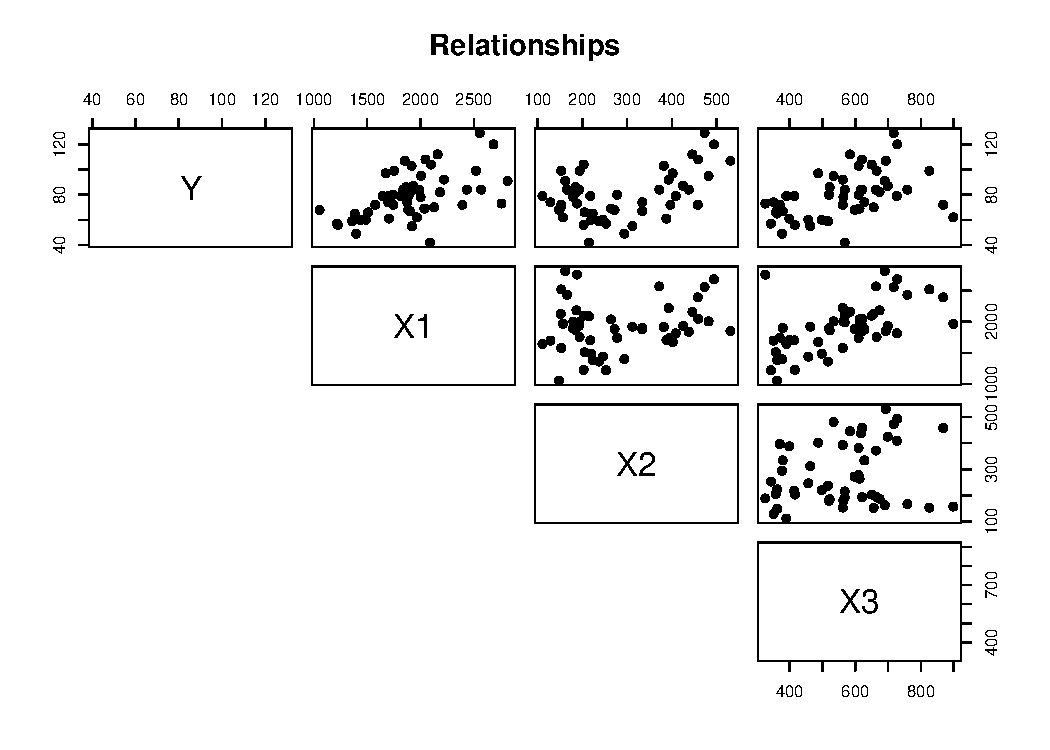
\includegraphics[width=\linewidth]{PS01_PT_YXXXplot.pdf}
\end{center}

\lstinputlisting[language=R, firstline=140, lastline=140]{PS01_PT.R}

\begin{verbatim}
	Y        X1        X2        X3
	Y  1.0000000 0.5317212 0.4482876 0.4636787
	X1 0.5317212 1.0000000 0.2056101 0.5952504
	X2 0.4482876 0.2056101 1.0000000 0.2210149
	X3 0.4636787 0.5952504 0.2210149 1.0000000
\end{verbatim}

\textbf{my interpretation of the graphs:}

Per capita expenditure on shelters/housing assistance in state (Y) displays a moderate positive correlation with all three variables of X. These X values being: per capita personal income in state (X1), Number of residents per 100,000 that are ”financially insecure” in state (X2), and Number of people per thousand residing in urban areas in state (X3). The relationship between Y and X1 has the most clear moderately positive correlation, while both the relationships between Y and X2 and Y and X3 have a moderately positive correlation with Y and X3 being slightly more strongly correlated. The correlations between X2 and X1 as well as X2 and X3 both have a weak positive correlation. The strongest correlation of all the plots is between X3 and X1 which shows a moderate positive correlation. There is one clear outlier that may be pulling the relationship away from a stronger correlation.


\item
\textbf{2.2} Please plot the relationship between \emph{Y} and \emph{Region}? On average, which region has the highest per capita expenditure on housing assistance?
\vspace{.5cm}

\textbf{my code:}
\lstinputlisting[language=R, firstline=158, lastline=166]{PS01_PT.R}

\begin{center}
	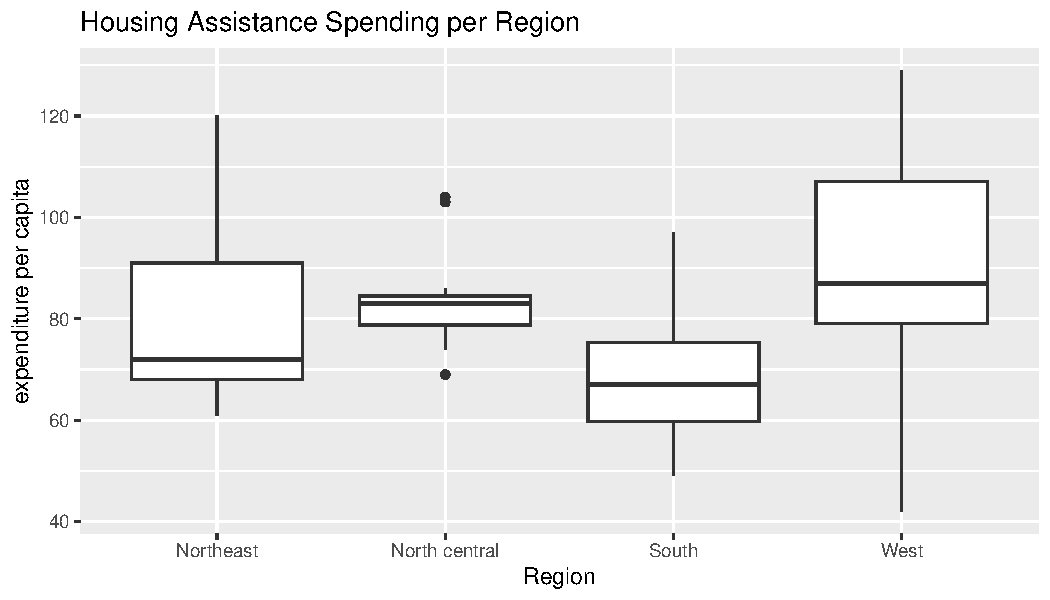
\includegraphics[width=\linewidth]{PS01_PT_boxplot.pdf}
\end{center}

\lstinputlisting[language=R, firstline=170, lastline=176]{PS01_PT.R}
\begin{verbatim}
	Northeast North_central         South          West 
	79.44444      83.91667      69.18750      88.30769 
\end{verbatim}

\textbf{my answer:}

On average the West had the highest per capita expenditure on housing assistance.

\item

\textbf{2.3} Please plot the relationship between \emph{Y} and \emph{X1}? Describe this graph and the relationship. 

\textbf{my code:}

\lstinputlisting[language=R, firstline=185, lastline=191]{PS01_PT.R}

\begin{center}
	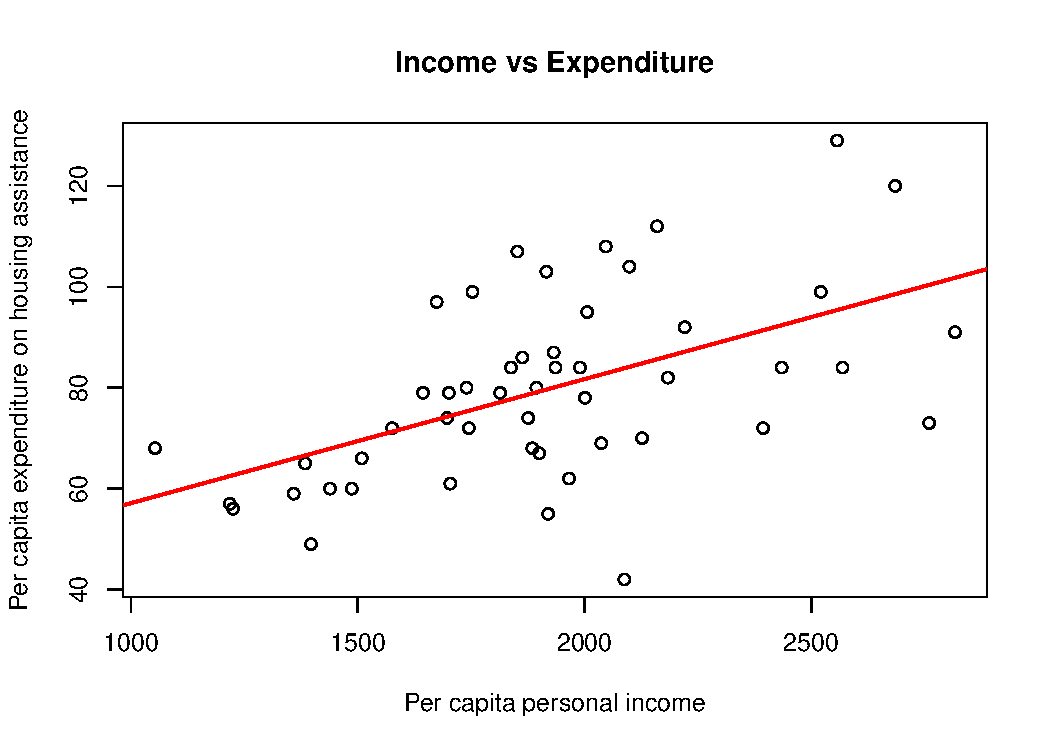
\includegraphics[width=\linewidth]{PS01_PT_YX1.pdf}
\end{center}

\lstinputlisting[language=R, firstline=195, lastline=195]{PS01_PT.R}
\begin{verbatim}
	[1] 0.5317212
\end{verbatim}

\textbf{my answer:}

  The graph shows that the per capita expenditure on shelters/housing assistance in state has a moderate positive correlation with per capita personal income in state. The points on the graph appear to begin landing further away from their predicted value more frequently as the values on the x and y axis get larger. A linear regression line was added to better visualize this.

\textbf{2.3.5} Reproduce the above graph including one more variable \emph{Region} and display different regions with different types of symbols and colors.

\textbf{my code:}
\lstinputlisting[language=R, firstline=208, lastline=220]{PS01_PT.R}
\begin{center}
	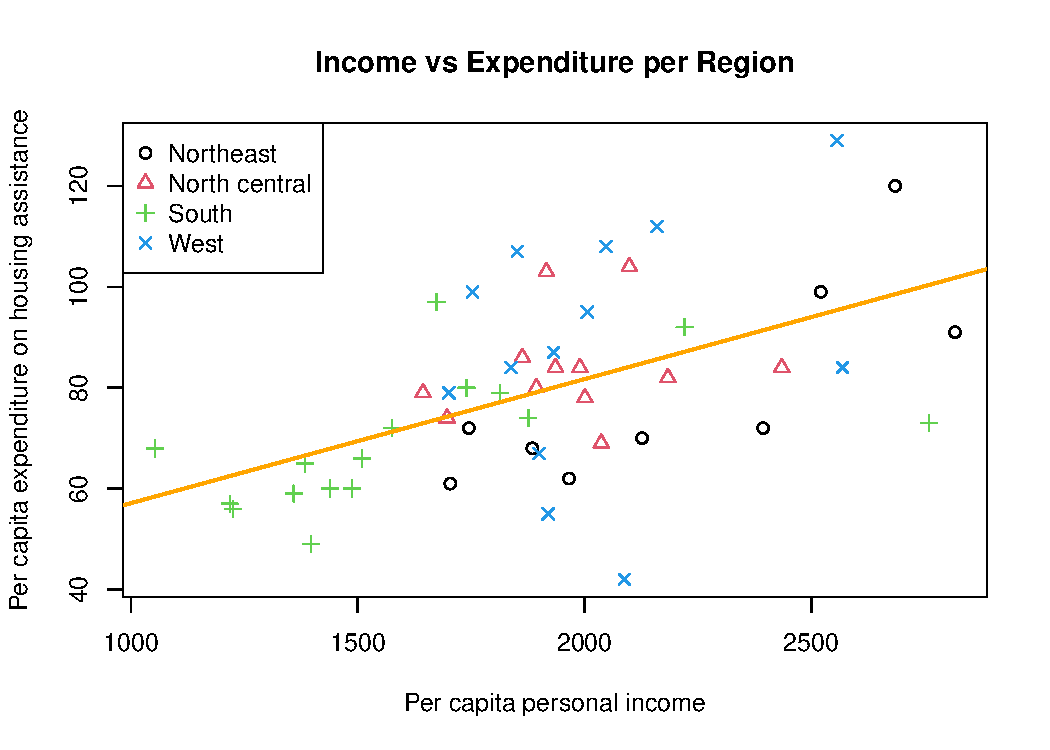
\includegraphics[width=\linewidth]{PS01_PT_YX1_colors.pdf}
\end{center}
\end{itemize}


\end{document}
